\documentclass[10pt,a4paper]{article}
\usepackage[utf8x]{inputenc}
\usepackage[T1]{fontenc}
%\usepackage{stringenc} % for grffile
\usepackage{ucs}
\usepackage{amsthm} %numéroter les questions
\usepackage[english]{babel}
\usepackage{datetime}
\usepackage{xspace} % typographie IN
\usepackage{hyperref}% hyperliens
\usepackage[all]{hypcap} %lien pointe en haut des figures
\usepackage[english]{varioref} %voir x p y
\usepackage{fancyhdr}% en têtes
%\input cyracc.def
\usepackage[]{graphicx} %include pictures
%\usepackage[encoding,inputencoding=utf8,filenameencoding=utf8]{grffile}
%\usepackage[extendedchars,inputencoding=latin1,filenameencoding=latin1]{grffile}
\usepackage[siunitx ]{circuitikz}
%\usepackage{gnuplottex}
\usepackage{ifthen}
\graphicspath{{./figures/}{./images/}}
\usepackage{array}
\usepackage{amsmath}
\usepackage[]{xcolor}
\usepackage{tikz}
\usepackage{tikz-timing}
\usetikzlibrary{scopes}
\usetikzlibrary{backgrounds}
\usepackage{listings}
\usepackage{enumitem}
\usepackage[top=1 in, bottom=1 in, left=1.3 in, right=1 in]{geometry} % Yeah, that's bad to play with margins
\usepackage[]{pdfpages}
\usepackage{pdflscape}
\usepackage[]{attachfile}
\usepackage{colortbl}
\usepackage{multirow}
\usepackage{booktabs}
\usepackage{rotating}
\usepackage{fontawesome} %Symbols
\usepackage{subcaption}

\newcommand{\version}{v1.0.0}

%cyr
%\newcommand\textcyr[1]{{\fontencoding{OT2}\fontfamily{wncyr}\selectfont #1}}


\newboolean{corrige}
%\setboolean{corrige}{true}%corrigé
\setboolean{corrige}{false}% pas de corrigé

\usepackage{aeguill} %guillemets

%% fancy header & foot
\pagestyle{fancy}
\lhead{[ELEC-H-473] Microprocessor Architectures: SIMD 2}
\rhead{\version\\ page \thepage}
\chead{\ifthenelse{\boolean{corrige}}{Corrigé}{}}
\cfoot{}
%%

\pdfinfo{
/Author (La saucisse électronique volante)
/Title (ELECH473 Lab 8 - SIMD 2)
/ModDate (D:\pdfdate)
}

\hypersetup{
pdftitle={ELECH473 Lab 8 - SIMD 2},
pdfauthor={Mouette unijambiste vengeresse},
pdfsubject={SIMD 1}
}

\theoremstyle{definition}% questions pas en italique
\newtheorem{Q}{Question}[] % numéroter les questions [section] ou non []

\newcommand{\reponse}[1]{% pour intégrer une réponse : \reponse{texte} : sera inclus si \boolean{corrige}
	\ifthenelse {\boolean{corrige}} {\paragraph{Réponse :} #1} {}
 }

\newcommand{\addcontentslinenono}[4]{\addtocontents{#1}{\protect\contentsline{#2}{#3}{#4}{}}}

\newcommand{\on}[1]{{\operatorname{#1}}}

\def\labelitemi{--}
\setlist{parsep=0pt,itemsep=0pt,style=standard,leftmargin=\parindent, align=left} % pas d'espace prohibitif entre les items
\setlist{nolistsep}

\newcolumntype{C}[1]{>{\centering\let\newline\\\arraybackslash\hspace{0pt}}m{#1}}

\setlength{\tabcolsep}{0pt} %no extra space in cells to keep constant tabular width

\date{\vspace{-1cm}\version}
\title{\vspace{-2cm} Lab 8\\ Microprocessor Architectures [ELEC-H-473]\\ SIMD 2: morphological image filtering \ifthenelse{\boolean{corrige}}{~\\Corrigé}{}}

%\author{\vspace{-1cm}}%\textsc{Yannick Allard}}


\lstdefinestyle{customasm}{
 % belowcaptionskip=1\baselineskip,
 % frame=L,
 % xleftmargin=\parindent,
 language=[x86masm]Assembler,
 basicstyle=\footnotesize\ttfamily,
 commentstyle=\itshape\color{magenta!40!black},
  comment=[l]//,
}

\lstset{escapechar=@,style=customasm}

\begin{document}

% Introduce a new counter for counting the nodes needed for circling
\newcounter{nodecount}
% Command for making a new node and naming it according to the nodecount counter
\newcommand\tabnode[1]{\addtocounter{nodecount}{1} \tikz \node (\arabic{nodecount}) {#1};}

% Some options common to all the nodes and paths
\tikzstyle{every picture}+=[remember picture,baseline]
\tikzstyle{every node}+=[inner sep=0pt,anchor=base]
\tikzstyle{every path}+=[thick, rounded corners]



\maketitle
\section*{Description of the lab}
This lab will focus on non-linear filtering algorithms that allows you to extract the contour of objects in an image or smooth imperfections.


Please refer to the course slides for an explanation about those filters.

\begin{figure*}[h]
    \centering
    \begin{subfigure}[t]{0.3\textwidth}
        \centering
        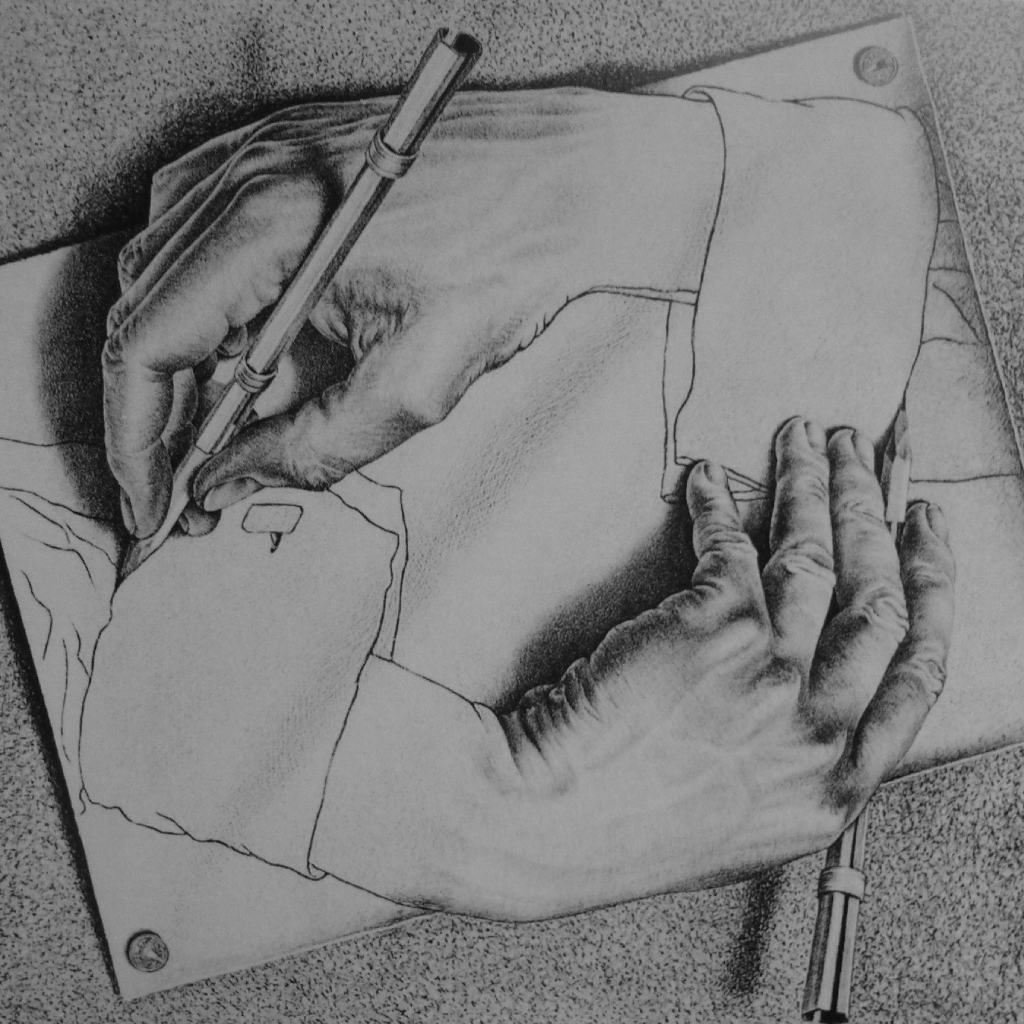
\includegraphics[height=4cm]{Escher.png}
        \caption{Reference image}
    \end{subfigure}%
    ~ 
    \begin{subfigure}[t]{0.3\textwidth}
        \centering
        \includegraphics[height=4cm]{out_3.png}
        \caption{3x3}
    \end{subfigure}%
    ~ 
    \begin{subfigure}[t]{0.3\textwidth}
        \centering
        \includegraphics[height=4cm]{out_5.png}
        \caption{5x5}
    \end{subfigure}
    \caption{Min/max filtering with different bouding box sizes.}
\end{figure*}

\section*{Assignment}
\begin{enumerate}
	\item Implement the min/max filtering (contour extraction) in C.
	Use at least a 3x3 bounding box. You can extend it to 5x5 and 7x7 as a bonus.
	\item Implement the same algorithm in SIMD.
	\item Benchmark both solutions and compare their performance.
\end{enumerate}

\subsection*{Code requirements}

\begin{itemize}
	\item Send only your source files, \textit{i.e.} .c/.h/.cpp/.hpp. Do \textit{not} send the input and output files.
	\item If your code requires specific configuration flags for the compilation, please write them down as comments in your code.
	\item Make sure it's well documented.
	\item All the input and output files should be in the source directory.
	\item All the output files should have the same base name as the source files on the UV (ie. Escher, kid or lena\_gray), appended with ``out\_C.raw'' or ``out\_SIMD.raw''.
	\item Do not use any weird library that may not compile on a Linux-based computer.
\end{itemize}


\end{document}
